% Section 3 - ROS 2 overview
% Roberto Masocco <roberto.masocco@uniroma2.it>
% April 23, 2025

% ### ROS 2 overview ###
\section{ROS 2 overview}
\graphicspath{{figs/section3/}}

% --- What is ROS 2? ---
\begin{frame}{What is ROS 2?}
	\begin{columns}
		\column{.5\textwidth}
		\only<1>{
			\nolistindent ROS 2 is a \textbg{DDS-based} (for now!), \textbg{open-source} middleware for robotic applications and software development.\\
			It allows developers to build and manage \textbg{distributed control architectures} made of many modules, usually referred to as \textbg{nodes}.\\
			\bigskip
			Its default DDS implementation is currently \textbg{Fast DDS} from \textbg{eProsima}.
		}
		\only<2>{
			\nolistindent \nolistindent ROS 2 currently supports \textbg{C++} and \textbg{Python} for application programming, and runs natively on \textbg{Ubuntu Linux 24.04}.
			\newline\newline
			New versions are periodically released as \textbg{distributions}: the current LTS one is \textbg{Jazzy Jalisco}; the development version is \textbg{Rolling Ridley} and can only be compiled from source.\\
			It is available as \textbg{binary \texttt{deb} packages} for \texttt{x86} and \texttt{ARMv8} architectures.
			\newline\newline
			A \textbg{distribution} is a collection of software packages: \textbg{libraries}, \textbg{tools}, and \textbg{applications}.
		}

		\column{.5\textwidth}
		\begin{figure}
			\centering
			
\includegraphics[width=.8\textwidth]{ros2Logo.jpg}
			\caption{ROS 2 logo.}
			\label{fig:ros2logos}
		\end{figure}
	\end{columns}
\end{frame}

% --- Why ROS 2? ---
\begin{frame}{Why ROS 2?}
	\begin{columns}
		\column{.5\textwidth}
		\only<1>{
			\nolistindent The ROS project started in 2005, to provide a middleware that could solve the \textbg{software integration} and \textbg{communication} problems in robotics. It has evolved much since then.
			\begin{block}{}
				\textbf{ROS is not an operating system in the traditional sense of process management and scheduling; rather, it provides a structured communications layer above the host operating systems of a heterogenous compute cluster.}
			\end{block}
      {\footnotesize Quigley, M. et al., \textbg{ROS: an open-source Robot Operating System}, ICRA workshop on open source software, 2005}
		}
		\only<2>{
			\nolistindent\nolistindent ROS 2 helps to design and build \textbg{distributed control architectures}, providing a common ground for the \textbg{integration} of different systems, sensors, actuators, and algorithms.\\
			It is a common framework for the development of \textbg{robotics software}.
			\newline\newline
			Its adoption is still limited because of familiarity with the original ROS, but it is \textbg{growing}.
		}

		\column{.5\textwidth}
		\begin{figure}
			\centering
			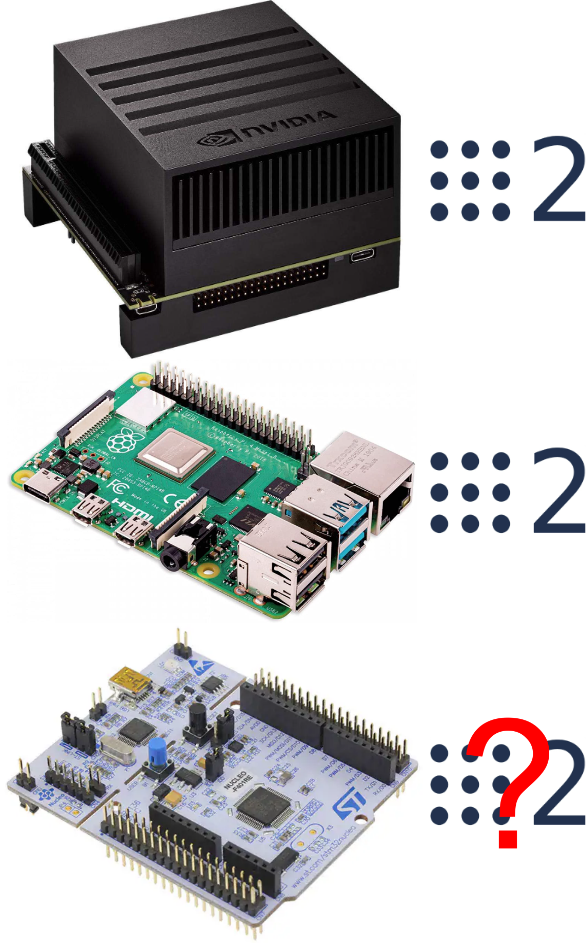
\includegraphics[scale=.17]{why_ros2.png}
			\label{fig:whyros2}
			\caption{STM32 (bottom), Raspberry Pi (middle), and Nvidia Xavier AGX (top).}
		\end{figure}
	\end{columns}
\end{frame}

% --- Main features ---
\begin{frame}{Main features}
	As a middleware, it offers many \textbg{services to roboticists}, including:
	\begin{itemize}
		\item \textbg{three communication paradigms}, easy to set up and based on the DDS (for now!): \textbg{messages}, \textbg{services} and \textbg{actions};
		\item organization of software packages, allowing for \textbg{redistribution and code reuse}, thanks to the \textbg{\texttt{colcon}} package manager;
		\item module configuration tools: \textbg{node parameters} and \textbg{launch files};
		\item integrated \textbg{logging subsystem} (involves both console and log files);
		\item CLI \textbg{introspection tools} for debugging and testing;
	\end{itemize}
\end{frame}
\begin{frame}{Main features}
	\begin{itemize}
		\item may be integrated in some \textbg{simulators} (\emph{e.g.}, Gazebo) and \textbg{visualizers} (\emph{e.g.}, RViz).
	\end{itemize}
	\begin{figure}
		\centering
		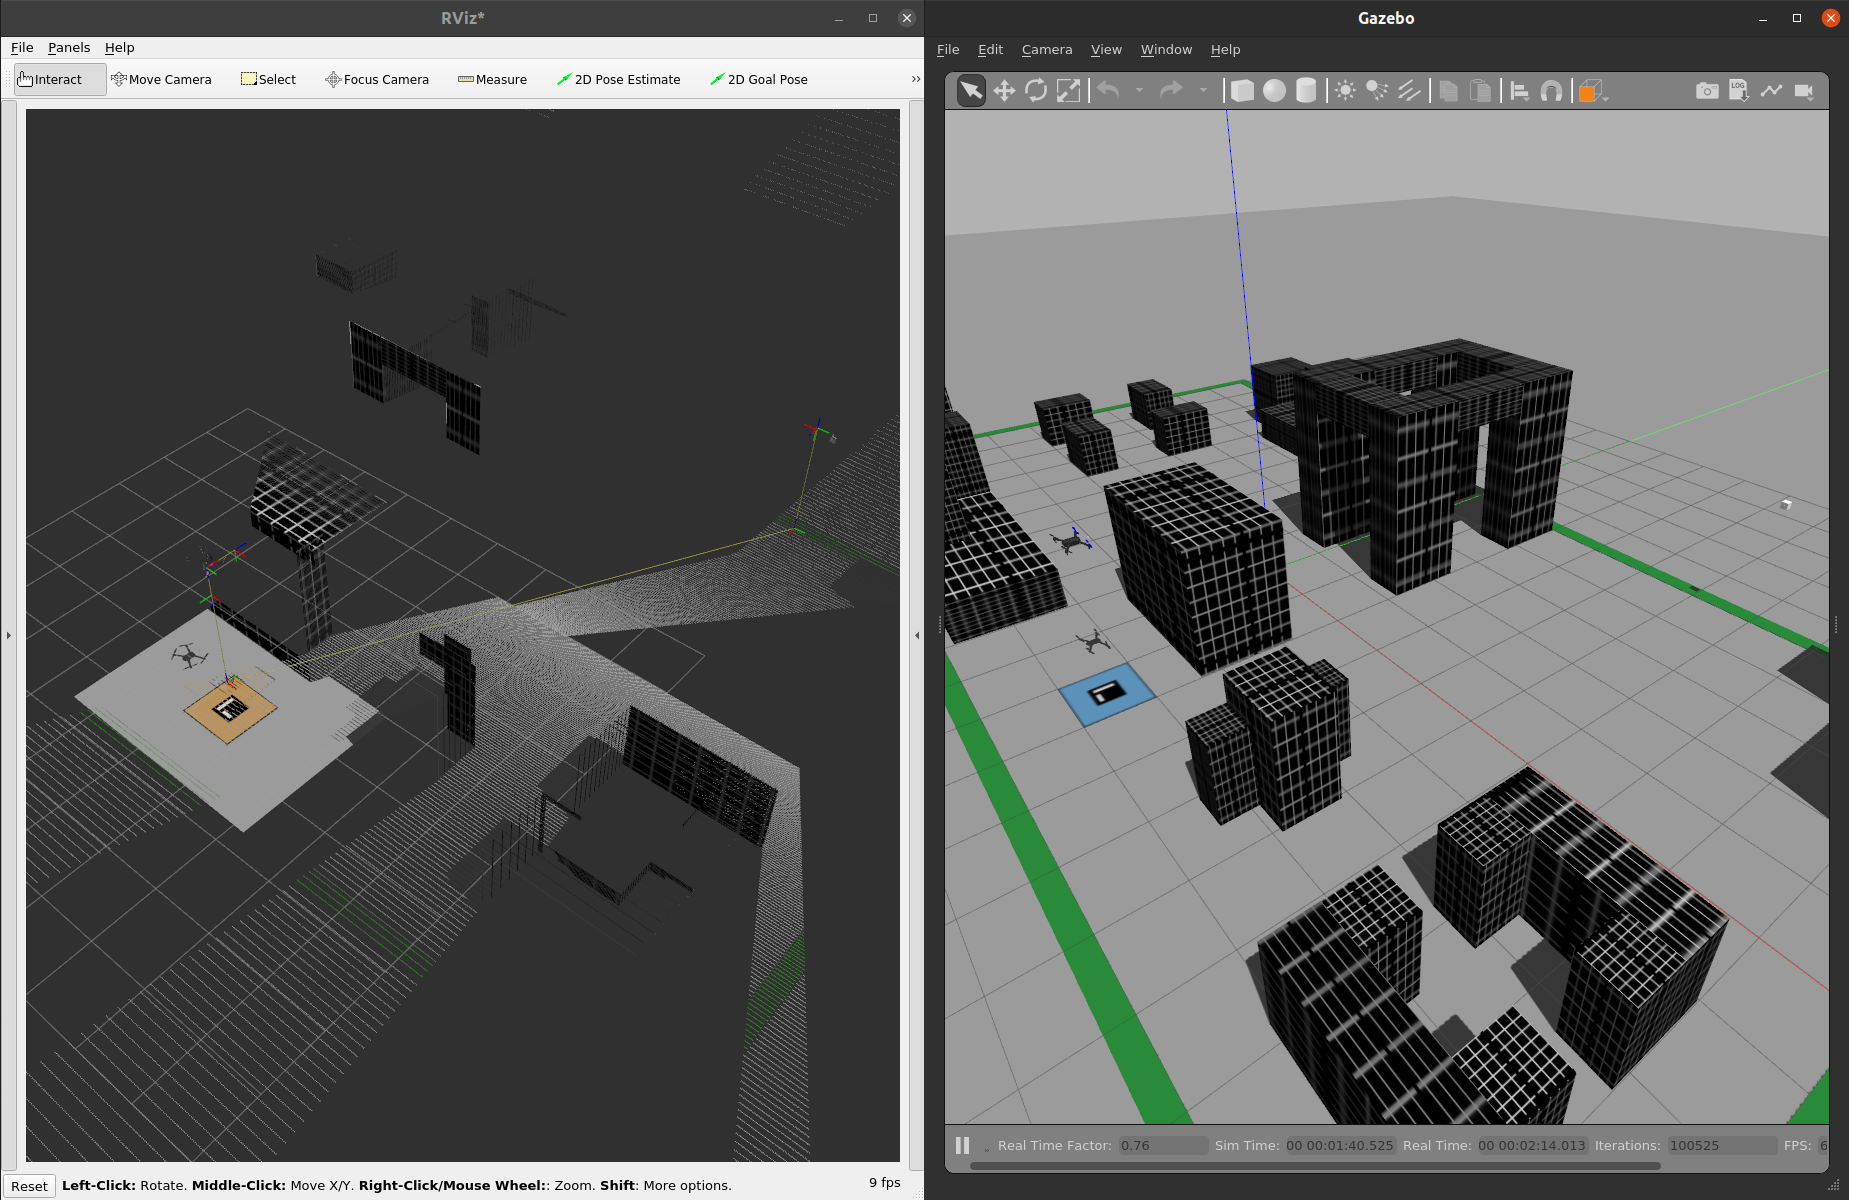
\includegraphics[scale=.133]{simulation.png}
		\label{fig:sim}
		\caption{Simulated drone in Gazebo Classic and RViz.}
	\end{figure}
\end{frame}

% --- The power of open source ---
\begin{frame}{The power of open source}
	The ROS project aims at establishing a common ground for the \textbg{development} of robotics just like what happened in the \textbg{software industry} in the last 30 years.\\
	\bigskip
	By \textbg{reusing code} and implementing \textbg{open hardware}, \textbg{building} a functioning robot may be only a matter of installing software, then writing four kinds of \textbg{text files}:
	\begin{itemize}
		\item \textbg{system files}, for onboard computers;
		\item \textbg{launch files}, to configure software startup and operation;
		\item \textbg{parameter files}, to set configuration parameters for software modules;
		\item \textbg{robot description files}, to tell the software how the robot is built;
	\end{itemize}
	even without a single line of code!\\
	\bigskip
	Open source enables quick \textbg{diffusion} and \textbg{improvement}, even on the \textbg{security} side, although new threats are rising: see the recent \href{https://en.wikipedia.org/wiki/XZ_Utils_backdoor}{\color{blue}\underline{\texttt{xz} backdoor}} case.
\end{frame}

% --- Application Programming Interface ---
\begin{frame}{Application Programming Interface}{Deep dive into ROS 2 internals}
	A \textbg{ROS 2 installation}, from bottom to top, works as follows:
	\begin{enumerate}
		\item \textbg{DDS}: the middleware that implements the \textbg{communication layer} (many different implementations are supported) (for now!).
		\item \textbg{RMW}: ROS MiddleWare, is the \textbg{DDS abstraction layer}, which allows to use different DDS implementations without changing the application code.
		\item \textbg{rcl}: ROS Client Support Library (C), implements basic entities: \textbg{nodes}, \textbg{publishers}, \textbg{subscribers}, \textbg{services}, \textbg{clients}, and \textbg{timers}.
		\item \textbg{rclc}/\textbg{rclcpp}/\textbg{rclpy}: ROS Client Library (C/C++/Python), implements the same entities as \texttt{rcl}, plus extended functionalities like the \textbg{executor}: a job scheduler.
	\end{enumerate}
	Then, there are \textbg{packages}: libraries, tools, and applications, both officially provided and community-contributed. The entire ROS 2 codebase is on \href{https://github.com/ros2}{\color{blue}\underline{GitHub}}.\\
	Keep this in mind during debugging, or while looking for information on an API!
\end{frame}
\begin{frame}{Application Programming Interface}{How a ROS 2 application works}
	The most important entity is the \textbg{node}, whose functionalities are specified upon creation.\\
	A node must usually do \textbg{a single thing}, being the \textbg{unit} in a \textbg{distributed architecture}.\\
	With its class methods, it can:
	\begin{itemize}
		\item act as an \textbg{entry point} towards the RMW layer, to handle communications;
		\item embed \textbg{software modules} like data, algorithms, and threads, that implement the application logic;
		\item register \textbg{callbacks} to handle \textbg{events}, such as timers or incoming messages.
	\end{itemize}
	Thus, it is both an \textbg{operational unit} and a \textbg{communication endpoint}.\\
	Nodes are usually handled by \textbg{executors}, which are responsible for scheduling and processing their \textbg{ROS-workload}.
	\begin{block}{}
		\centering
		\textbf{Nodes are just objects in your application: they can embed any kind of software module, but they do not limit your design to their paradigms.}
	\end{block}
\end{frame}

% --- Executors: events and callbacks ---
\begin{frame}{Executors}{Handling events and callbacks}
	\begin{figure}
		\centering
		\includesvg[scale=.45]{ROS2_executor_scheme.svg}
		\label{fig:executorscheme}
		\caption{ROS 2 event-based programming paradigm.}
	\end{figure}
\end{frame}
\begin{frame}{Executors}{Handling events and callbacks}
	\begin{enumerate}
		\item Middleware functionalities trigger \textbg{(a)synchronous events}.
		\item Events are handled by \textbg{background jobs}, coded in \textbg{callbacks} by the programmer.
		\item Callbacks are \textbg{registered} into a \textbg{node} when its functionalities are specified (\emph{e.g.}, upon creation).
		\item The workload that a node carries is scheduled and processed by an \textbg{executor}, single- or multi-threaded.
	\end{enumerate}
	\begin{alertblock}{}
		\centering
		Executors implement a \textbr{round-robin}, \textbr{non-preemptive} policy that \textbr{always prioritizes timers}.
	\end{alertblock}
\end{frame}

% --- Flaws ---
\begin{frame}{Flaws}{The devil is in the details}
	\visible<1->{
		\begin{alertblock}{ROS 2 main design flaws as of today}
			The main concerns arise when developing low-level stuff:
			\begin{itemize}
				\item \textbr{the DDS/RMW layer is almost completely abstracted}, so non-standard network or DDS configurations may get tricky;
				\item the internal job scheduling algorithm (namely the \textbr{executor}) is \textbr{not suited for hard real-time applications} because of its \textbr{non-preemptive} nature.
			\end{itemize}
		\end{alertblock}
	}
	\visible<2>{
		What to do when development gets to a really low level?
		\begin{itemize}
			\item Hand off stuff to dedicated \textbg{microcontrollers}.
			\item Use \textbg{micro-ROS}: hard real-time ROS 2 on microcontrollers and different communication interfaces.
		\end{itemize}
	}
\end{frame}
\begin{frame}{Flaws}{The DDS layer abstraction}
	ROS 2 nodes can either \textbg{publish to} or \textbg{subscribe to} a \textbg{topic}.
	\begin{block}{Definition of ROS 2 topic}
		A ROS 2 topic is \textbf{uniquely identified} by three attributes:
		\begin{itemize}
			\item a \textbf{name}, \emph{i.e.}, a human-readable character string;
			\item an \textbf{interface}, \emph{i.e.}, a custom packet format that specifies what data is carried over it (\emph{e.g.}, strings, numbers, arrays...);
			\item a \textbf{single QoS policy} that specifies how transmissions should be performed.
		\end{itemize}
	\end{block}
	\begin{block}{}
		\centering
		\textbf{Changing even only one of the above results in a completely different topic!}
	\end{block}
	Compare this to the DDS way of setting up a communication channel between two applications...
\end{frame}
\begin{frame}{Flaws}{The DDS in a multi-agent environment}
	Over the years, ROS 2 helped identify some \textbg{flaws} in the \textbg{DDS standard}:
	\begin{itemize}
		\item communication with \textbg{large data} (\emph{e.g.}, images, pointclouds...) over a \textbg{lossy network} becomes inefficient or impossible, due to \textbg{retransmission policies};
		\item \textbg{discovery} of \textbg{many endpoints}, especially over a \textbg{lossy network}, may become slow or \textbg{clog} the network completely, due to the amount of generated \textbg{traffic}.
	\end{itemize}
	Just think about a \textbg{swarm} of drones, each one cameras and the like, trying to communicate over a \textbg{wireless network}...
\end{frame}
\begin{frame}{Flaws}{Abandoning the DDS?}
  ROS 2 steering committees are considering the \textbg{abandonment} of the DDS middleware in favor of \textbg{new solutions}.\\
  The main requirements are:
  \begin{itemize}
    \item \textbg{scalability}, especially with entity queries;
    \item \textbg{low latency}, on constrained hardware and low-power networks;
    \item \textbg{configurability};
    \item \textbg{optimization of data transfers}.
  \end{itemize}
  \bigskip
  The newest LTS version, \textbg{Jazzy Jalisco}, is the first one to ship with a RMW based on the \href{https://zenoh.io/}{\color{blue}\textbf{\underline{Zenoh}}} middleware.
\end{frame}

% --- Zenoh ---
\begin{frame}{Zenoh}
	\begin{columns}
		\column{.5\textwidth}
		\textbg{Zenoh} is a new middleware for distributed communication meant as a \textbg{successor of the DDS}.\\
		It is designed to handle \textbg{three main types of data:}
		\begin{itemize}
			\item \textbg{data in motion} that is being transmitted over the network;
			\item \textbg{data at rest} that is stored in a device and can be retrieved at any time;
			\item \textbg{data for computations} as in remote procedure calls.
		\end{itemize}
		It relies on a \textbg{router daemon} (\texttt{zenohd}).

		\column{.5\textwidth}
		\begin{figure}
			\centering
			
\includegraphics[width=.65\textwidth]{zenoh}
			\label{fig:zenoh}
			\caption{Zenoh logo.}
		\end{figure}
	\end{columns}
\end{frame}
\begin{frame}{Zenoh}
	\begin{figure}
		\centering
		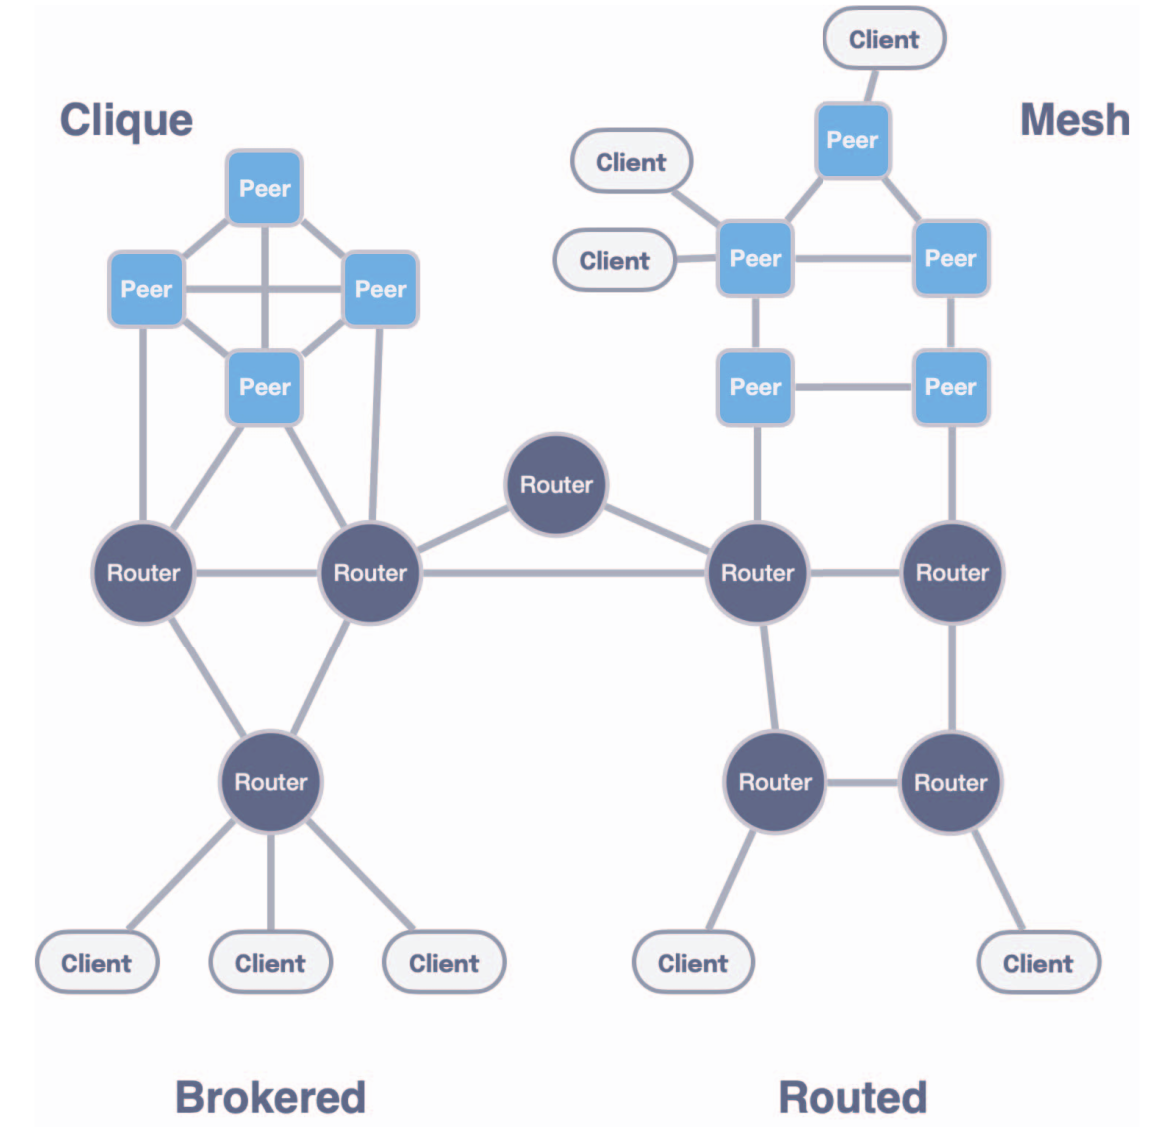
\includegraphics[width=.45\textwidth]{zenoh_networks}
		\label{fig:zenohnets}
		\caption{Possible network configurations in Zenoh.}
	\end{figure}
\end{frame}
